\documentclass[../Immersed_Boundary_Method.tex]{subfiles}

\begin{document}


\section{Simulating the Poiseuille Flow}

Poiseuille's FLow describes a laminra steady flow of an incompressible \textbf{viscous} fluid through a cylindrical pipe with a constant cross-section.

\subsection{The Parabolic Velocity Profile}
\begin{center}
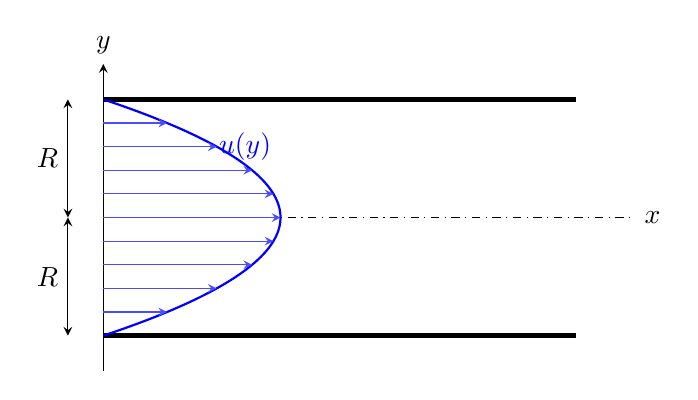
\begin{tikzpicture}[scale=1.5, >=stealth]
    % Pipe Walls
    \draw[ultra thick] (0, 1) -- (4, 1);
    \draw[ultra thick] (0, -1) -- (4, -1);

    % Centerline and Axis
    \draw[dash dot] (0,0) -- (4.5,0) node[right] {$x$};
    \draw[->] (0,-1.3) -- (0,1.3) node[above] {$y$};

    % Parabolic Velocity Profile
    \draw[blue, thick, domain=-1:1, samples=100] plot ({1.5*(1-\x*\x)}, \x);

    % Velocity Vectors
    \foreach \y in {-0.8,-0.6,-0.4,-0.2,0,0.2,0.4,0.6,0.8} {
        \draw[->, blue!70] (0,\y) -- ({1.5*(1-\y*\y)}, \y);
    }

    % Labels
    \node[blue] at (1.2, 0.6) {$u(y)$};
    \draw[<->] (-0.3,0) -- node[left] {$R$} (-0.3,1);
    \draw[<->] (-0.3,0) -- node[left] {$R$} (-0.3,-1);
\end{tikzpicture}
\end{center}
We use cylinder coordinate and set 
\[ \bm{u} = (u_r, u_\theta, u_z) = (u_r, u_\theta, w) = (u_r, 0, w(r))\]
Idealy, the velocity is zero at the wall, i.e. $w(R) = 0$. 
From the \textbf{Mass Conservation}
\begin{equation}
\nabla \cdot \bm{u} = w_z + \frac{1}{r} (r u_r)_r + \frac{1}{r} u_\theta = 0
\end{equation}
Since $w$ is constant in $z$ direction, then $w_z =0$, so we have $u_r = 0$. Now by newtonian law in $r$ direction. 
\[ \frac{p_r}{\rho} = 0 \qrq p = p(z)\]
The pressure only depends on $z$ direction. Now since 
\[ \Delta w = \frac{1}{r}(rw_r)_r\]
Then the $z$ component of the N-S equation is 
\[ \frac{P_z}{\rho} = \mu \frac{1}{r}(r w_r)_r\]
Then using the boundary condition $w(R) = 0$, we have 
\begin{equation}
\boxed{w(r) = \frac{P_z}{4\mu}(r^2-R^2)}
\end{equation}
This is the velocity profile for the Poiseuille Flow. \par
\subsubsection{Reynolds Number}
The existence of the parabolic velocity profile is based on the assumption that the flow is viscous. The Reynolds number should be small in order to neglect the inertial term. 
\begin{equation}
Re = \frac{\rho U D}{\mu} < 2000
\end{equation}
For a standard case, let's compute the Reynolds number explicitly. Let's look at a biological example: how much a small amount of plaque buildup affects blood flow in an artery. The constants : 
\begin{enumerate}
    \item Length of artery section ($L$): 0.05 meters
    \item Pressure Drop ($\Delta P$): 400 Pascals (the force from the heart)
    \item Viscosity of blood ($\eta$): 0.004 Pa·s
    \begin{enumerate}
        \item Healthy Artery ($R_1$): Has a radius of 0.002 meters (2 mm).
        \item Narrowed Artery ($R_2$): Plaque has reduced the radius by just 20\%, making it 0.0016 meters (1.6 mm).
    \end{enumerate}
\end{enumerate}
\subsubsection{Total Flux}
The average velocity is given by 
\[ \bar{w} = \frac{1}{\pi R^2} \int_{0}^{R}2\pi r \frac{P_z}{4\nu}(R^2 - r^2)dr = \frac{P_z R^2}{8\nu}\]
Now since we are adding a constant force $F$ on the right boundary of the tube, then 
\[ P_z = \frac{F}{\pi R^2} \cdot \frac{1}{L}\]
Where $L$ is the length of the tube. Then we have 
\[ \bar{w} = \frac{F}{8 \pi L \nu}\]
Formula to the Reylolds number for this system is approximatedly 
\[ \text{Re} = \frac{\rho \bar{w} R}{\nu} = \frac{\rho F}{8 \pi L \nu^2}\]

\subsection{2D Poiseuill's Flow}
Now imagine we have a 2D channel with length $L$ and radius $R$. What is the velocity profile in this case? Starting from mass conservation. 
\[ \nabla \cdot \bm{u} = u_x + v_y = 0 \qrq u_x = 0\]
The Newtonian law in $x$ direction is 
\[ \frac{p_x}{\rho} = \nu \Delta u = \nu u_{yy}\]
Since $u_x = 0$, integrate the equation and use the boundary condition $u(-R) = u(R) = 0$, we have 
\begin{equation}
 \boxed{u(y) = \frac{p_x}{2\nu}(y^2 - R^2)}
\end{equation}
Since $p$ decreases so $p_x < 0$, then the sign is positive. 




\end{document}